%% The first command in your LaTeX source must be the \documentclass command.
%%
%% Options:
%% twocolumn : Two column layout.
%% hf: enable header and footer.
\documentclass[
% twocolumn,
hf, % comment this for submission
]{ceurart}

%%
%% One can fix some overfulls
\sloppy

%%
%% Minted listings support 
%% Need pygment <http://pygments.org/> <http://pypi.python.org/pypi/Pygments>
\usepackage{listings}
\usepackage{todonotes}
\usepackage{import}
\usepackage{graphicx}
\usepackage{multirow}
\usepackage{graphicx}
%\usepackage{rotating}
\usepackage{float}
\usepackage[figuresleft]{rotating}

%% auto break lines
\lstset{breaklines=true}

%%
%% end of the preamble, start of the body of the document source.
\begin{document}

%%
%% Rights management information.
%% CC-BY is default license.
\copyrightyear{2022}
\copyrightclause{Copyright for this paper by its authors.
  Use permitted under Creative Commons License Attribution 4.0
  International (CC BY 4.0).}

%%
%% This command is for the conference information
\conference{International Workshop on Knowledge Graph Summarization (KGSum), December 5--7, 2023, Pensacola, Florida, USA}

%%
%% The "title" command
\title{From Nodes to Narratives: A Knowledge Graph-based Storytelling Approach}

\author[1]{Author 1}[%
 email=name.surname@institution1.org,
]
\cormark[1]

\author[2]{Author 2}[%
  email=name.surname@institution2.org,
]
\cormark[1]

\author[2]{Author 3}[%
  email=name.surname@institution2.org,
]

\address[1]{Institution 1, City 1, Country 1}

\address[2]{Institution 2, City 2, Country 2}

%%
%% The "author" command and its associated commands are used to define
%% the authors and their affiliations.
% \author[1,2]{Mike de Kok}[%
%  orcid=0009-0009-9843-4707,
% email=m.a.h.de.kok@student.vu.nl,
% % url=https://yamadharma.github.io/,
% ]
% \cormark[1]

% \author[2]{Youssra Rebboud}[%
%   orcid=0000-0003-3507-5646,
%   email=youssra.rebboud@eurecom.fr,
% ]
% \cormark[1]


% \author[2]{Pasquale Lisena}[%
%   orcid=0000-0003-3094-5585,
%   email=pasquale.lisena@eurecom.fr,
% ]
% \author[2]{Raphael Troncy}[%
%   orcid=0000-0003-0457-1436,
%   email=raphael.troncy@eurecom.fr,
% ]

% \author[1]{Ilaria Tiddi}[%
% orcid=0000-0001-7116-9338,
% email=i.tiddi@vu.nl,
% % url=https://kmitd.github.io/ilaria/,
% ]

% \address[1]{Vrije Universiteit Amsterdam, Amsterdam, The Netherlands}


% \address[2]{EURECOM, Sophia Antipolis, France}



%% Footnotes
\cortext[1]{Corresponding author.}

%%
%% The abstract is a short summary of the work to be presented in the
%% article.
\begin{abstract}
Narratives wield a profound influence, shaping perceptions, beliefs, and decision-making processes. Although contemporary pre-trained language models have showcased impressive capabilities in text generation and question-answering tasks, they grapple with inherent limitations in knowledge coverage and exhibit vulnerability to societal biases. This work endeavors to forge a methodology that applies knowledge graphs in narrative construction. Rather than solely focusing on fundamental aspects such as the 4W (who, what, when, where) and general relationships, our approach comprises finely detailed semantic relations, delineating precise type of causality such as an event preventing, intending-to-cause, causing, or enabling another event. Applying state-of-art methods to predict such rich information, we demonstrate that it is possible to obtain automatically generated narratives of better grammatical and semantic accuracy.
\end{abstract}

%%
%% Keywords. The author(s) should pick words that accurately describe
%% the work being presented. Separate the keywords with commas.
\begin{keywords}
 Narratives\sep
 Knowledge Graphs \sep
 Information Extraction  \sep
 Event-centric Knowledge Graphs
\end{keywords}

%%
%% This command processes the author and affiliation and title
%% information and builds the first part of the formatted document.
\maketitle

\section{Introduction}
\label{sec:introduction}
Narratives stand at the heart of our societal fabric, serving our understanding and facilitating the exchange and preservation of knowledge. These narratives filter through our everyday lives, appearing in diverse forms such as commercials, political campaigns, news broadcasts, and more, each with its unique purpose and significance. 
Stories hold immense power to shape our thoughts, beliefs, and actions, making them captivating and transformative~\cite{green2004understanding}. Consequently, the quest to innovate in the realm of complex narrative generation holds the potential to usher in a new era of AI systems that are intricately attuned to human sensibilities. Building upon the profound role of narratives in our society, it becomes evident that our means of narrative generation and comprehension are intertwined with the capabilities of modern AI. Pre-trained large language models, exemplified by models such as BERT \cite{BERT}, GPT-3 \cite{GPT-3}, and the more recent ChatGPT (GPT-3.5)\footnote{\url{https://openai.com/blog/chatgpt/}}, have showcased remarkable progress in text generation, and conversational tasks. Yet, these models, shaped by training on extensive datasets drawn from undisclosed and diverse sources, bear intrinsic limitations, including knowledge gaps, inaccuracies, and societal biases \cite{GPT-3,documenting_corpora}. Their challenges in maintaining semantic coherence and capturing long-term dependencies within text generation further underscore the need for innovation in narrative crafting \cite{PLM_survey,semantic_coherence}. 

Knowledge Graphs (KGs) are proven to be suitable structures for human knowledge, designed for machine-readability and adaptability, while several experiments of text generation from KGs are present in the literature \cite{KG_survey}. Several KGs are available as data sources for the automatic generation of narratives. For example, \textit{EventKG} \cite{gottschalk2019eventkg} is a knowledge graph that consolidates and links events extracted from diverse sources, including Wikidata and YAGO \cite{hoffart2013yago2}. This knowledge graph comprises more than 1.3 million events, each associated with its respective spatial and temporal coordinates. However, EventKG primarily focuses on representing events attributed and relationships between sub-events and super-events. While the value of such a knowledge graph is undeniable, its limitation to specific event properties, notably the sub(super)events or the 4W, results in succinct and somewhat incomplete narratives. To address this limitation, we propose enriching this information by incorporating detailed event relations~\cite{beyond_causality}.

The FARO dataset~\cite{beyond_causality,sem_data_aug} encompasses a broader spectrum of semantically precise relationships. This includes event-related connections such as \textit{Prevention}, \textit{Enabling}, \textit{Causality}, and \textit{Intention}. In this work, we propose to enhance the WebNLG dataset~\cite{gardent-etal-2017-creating}, by incorporating the FARO dataset. This expansion aims to produce more linguistically sophisticated generated text with richer semantic content.

The remainder of this paper is structured as follows: we first review the prior research pertaining to narratives and the extraction of relevant information from KGs (Section~\ref{sec:related-work}). We present datasets in Section~\ref{sec:dataset}, and we detail our approach for KG summarization, which encompasses an initial information selection step before text generation in Section~\ref{sec:KGS}. We then present both qualitative and quantitative results in Section~\ref{sec:results_jointGT}. We conclude and outline some future work in Section~\ref{sec:conclusion}.

\section{Related Work }
\label{sec:related-work}
A \textit{narrative graph} \cite{Build_narrative} incorporates two main components: the individual representation of events, including the ``four W" aspects (\textit{who}, \textit{what}, \textit{when}, \textit{where}) and the interconnection of these events through temporal and causal relationships. The \textit{Simple Event Model} (SEM) \cite{SEM} provides a foundation for modeling events, but is still insufficient to link disparate events or classes of the same type. To address this limitation, \citeauthor{Build_narrative} \cite{Build_narrative} suggests enriching the event relation types: temporal or causal links from \citeauthor{allen} \cite{allen} and \texttt{dbo:alongside} links between classes of the same type. Furthermore, the FARO ontology\footnote{\url{https://anr-kflow.github.io/faro/}}~\cite{beyond_causality} covers most of the existing event relations in the literature, from temporal relation to causal and more fine-grained ones such as \textit{prevention}.

KG summarization is an initial step of information retrieval and selection. To acquire the essential nodes for event description, an effective approach involves ranking techniques that assign significance to nodes based on the relationships they possess. Various methods can be used such as entity ranking, relationship ranking, and semantic document ranking \cite{JINDAL2014416}. \cite{graph_traversal} proposes a system that can identify relevant information needed to build a narrative graph, by using an informed graph search traversal strategy. To determine which information is considered 'relevant' the method uses filters to prune the search space with respect to the Simple Event Model (What, Who, Where, When).

On the other hand, different methods for generating texts from knowledge graphs have been proposed. In \cite{creative_story}, triples are extracted to fine-tune a GPT-2 model \cite{GPT-2}, making the model dependent on the input triples. A similar approach is introduced in \cite{inv_PLM}, involving BART~\cite{BART} and T5~\cite{T5}. This approach obtained state-of-the-art performances on the AGENDA dataset \cite{AGENDA_KG} but not on the WebNLG dataset. Both found that Pre-trained Language Models (PLM) work well on unordered representations of the graph. JointGT~\cite{JointGT} uses BART and T5, and exploits new pre-training methods to explicitly preserve the input graph's structural information. JointGT outperforms the other mentioned technique on WebNLG, which might indicate that including the topology of the graph lead to better results. A different approach~\cite{DRAW} uses a transformer encoding structure to encode both the global information and the local topology information, and feeds a transformer to decode and generate text. However, this did not work as well as the previously mentioned technique \cite{inv_PLM}, which used a PLM model without encoding. This might indicate that PLMs obtain better results than self trained transformer models.

\section{Dataset} 
\label{sec:dataset}
In this section, we present the datasets that will be used to train our method: WebNLG~\cite{WebNLG}, the FARO dataset~\cite{sem_data_aug} (Table \ref{tab:rebel_data}). For evaluation, we use two evaluation datasets: the FARO test set and the ASRAEL KG~\cite{ASRAEL}. ASRAEL is a knowledge graph that includes various event-related articles and their interconnections, including the 4W relations.

\begin{table}[htbp]
  \resizebox{\textwidth}{!}{  
\begin{tabular}{|l|l|l|l|l|}
\hline
\textbf{Sentence}                                    & \textbf{Trigger1} & \textbf{Trigger2} & \textbf{Tag} & \textbf{Triplets}                     \\ \hline
\begin{tabular}[c]{@{}l@{}}The government has implemented a series\\ of laws to prevent the abuse of animals.\end{tabular} & laws              & abuse             & prevent      & \begin{tabular}[c]{@{}l@{}}\textless{}triplet\textgreater laws \textless{}subj\textgreater\\  abuse \textless{}obj\textgreater prevent\end{tabular} \\ \hline
\end{tabular}
}
\caption{Sample of the FARO dataset}
\label{tab:rebel_data}
\end{table}

We enhanced the ASRAEL KG with additional relations (similarly to the ones in FARO) within its articles, resulting in a more intricate and comprehensive knowledge graph. To achieve this objective, we used the REBEL model \cite{REBEL} to extract event mentions and event relations. Furthermore, we leverage an existing event co-reference resolution model~\cite{barhom-etal-2019-revisiting} to perform the task within the KG. This model creates clusters of mentions, computes similarity scores for each cluster, merges those with the highest score, and repeats this process until the score fell below a defined threshold, which we empirically set to 0.95. This clustering process resulted in a graph primarily composed of single mentions. Syntactic matches within these clusters were notably high, indicating the quality of our co-reference resolution. In total, we successfully clustered 45,031 mentions, with 36,057 being unique. The resulting narrative graph\footnote{
% \url{https://github.com/ANR-kFLOW/KG2Narrative/blob/main/Data/graphs/final_generated/eag_complete_merged.ttl}
\url{https://anonymous.4open.science/r/KG2Narrative/Data/graphs/final_generated/eag_complete_merged.ttl}
} provides a RDF representation of event co-references and relationships, enriched with ontologies such as NIF (NLP Interchange Format\footnote{\url{https://persistence.uni-leipzig.org/nlp2rdf/}}), SEM and FARO to describe the relations between triples, further enhancing the context and meaning of our knowledge graph. More detailed information can be found in Appendix \ref{sec:appendix}.

\section{Knowledge graph summarization}
\label{sec:KGS}
Knowledge Graph summarization comprises two tasks: the selection of pertinent information from the knowledge graph, and the text generation based on the extracted data.

\paragraph*{Relevant Information Selection}
%We have implemented a graph search algorithm tailored to the identification of essential nodes for the narrative. This algorithm, in alignment with a predefined heuristic, prioritizes the selection of the most critical nodes corresponding to the 4W, which we identify as necessary for describing the narrative. Narrative filters have been established in accordance with SEM, encompassing the 4W.
% Upon the activation of a filter to filter out certain properties, nodes of that particular property are disregarded during the search process.
%The \textit{expansion} of a node is defined as retrieving the nodes directly connected to the selected node. The algorithm's operational sequence comprises the following steps:
%\begin{enumerate}
% \item initialise a sub-graph \textit{SG};
% \item initialise pending nodes \textit{PN}, by adding a defined starting node to it;
% \item compute scores for nodes in \textit{PN}, using the \textit{Predicate Object Frequency} heuristic;\footnote{Edges containing the tuple (predicate, object) that are frequently used in the graph will be preferred.}
% \item expand nodes with the highest ranking; %Not sure what threshold (could not find it in graph search paper)
% \item apply the narrative filters on retrieved nodes, keeping only the relevant nodes;
% \item add the relevant nodes to \textit{PN}, and to the output \textit{SG};
% \item Repeat steps 3 to 6 until the maximum number of iterations is reached.
%\end{enumerate}

%We use the "predicate object frequency" heuristic, this builds on the assumption that if an entity has many links to it, it indicates it is more relevant. The predicate \texttt{schema:about} is filtered out, since there already exists a link between the article and the event (with \texttt{schema:subjectOf}).
% To test the model, initially, the event ``2021 storming of the United States Capitol" has been chosen (start node). This event is, as the name suggests, about the storming of the Capitol in the United States. This event contains the 4W, and is the subject of 65 news articles.

%During preliminary tests on a subset of events, we found that the node expansion easily includes other events than the starting one, because many events and articles that link to the same places, times, etc. are eventually included in the expansion. This may lead to an extracted subgraph that is not strictly focused on the original event of interest. In particular, some mentions\footnote{Sub-events in a narrative graph, see \textit{trigger1}, \textit{trigger2} in Table \ref{tab:rebel_data}.} may not be expanded, since the algorithm may pick another path. To overcome this issue, a SPARQL query has been used to retrieve the most important 4W nodes, according to the \textit{Predicate Object Frequency}.

A SPARQL query has been used for the identification of essential nodes for the narrative. This query, prioritizes the selection 4W nodes, with a higher frequency of incoming edges. Mentions are selected similarly; the larger the cluster of identical mentions that were formed by the event co-reference model is, the higher the priority of said cluster. Since we face a limitation on the number of input tokens of the text generation model, up to three mentions are selected from different clusters.

The quality of the output depends largely on the quality the output of previous steps (relation extraction and co-reference resolution). Future work aims to enhance the accuracy of both these tasks and explore methods for identifying indirectly linked relevant nodes to selected events.


\subsection{Text Generation from Knowledge Graphs}
As anticipated in Section \ref{sec:related-work}, using a PLM instead of training a language model from scratch can lead to better results. Furthermore, incorporating the graph's topology into the model has been shown to generate better natural text. The JointGT model \cite{JointGT} incorporates both these characteristics, hence, we adopted this method. The authors pre-trained this model on the KGText dataset~\cite{KGtext}, consisting of 7 million graph-text pairs extracted from the English Wikidump.\footnote{\url{https://dumps.wikimedia.org/}} It includes around 1.8 million entities and 1,210 relations.

The WebNLG dataset does not contain any of the FARO relations. Therefore, we fine-tuned the model on a merged dataset, combining the WebNLG and FARO, as in Table \ref{tab:splits_dataset_jointgt}.

\begin{table}[h]
\caption{Sizes of the datasets used for training and evaluating the JointGT model}
\centering
\begin{tabular}{|l|r|r|r|}
\hline
\textbf{Dataset} & \textbf{Train} & \textbf{Val} & \textbf{Test} \\ \hline
WebNLG           & 12,876          & 1,619         & 1,600          \\ \hline
FARO             & 1,800           & 201          & 108            \\ \hline
Combined         & 14,676          & 1,820         & 1,708          \\ \hline
\end{tabular}

\label{tab:splits_dataset_jointgt}
\end{table}

The model undergoes fine-tuning on the WebNLG dataset. We refer to the original model as \textit{base model}, and the model fine-tuned on the combined dataset as \textit{combined model}.\footnote{The model was replicated using the same parameters from the original paper, except for the batch size lowered due to memory constraints. The parameters are \textit{Learning rate}: 0.000025, \textit{Batch size}: 4, \textit{Epochs}: 10, \textit{Optimizer}: Adam. \textit{Early stopping}: 10 epochs}

\section{Results}
\label{sec:results_jointGT}

\subsection{Quantitative analysis}
%Maybe make it more clear that also testing was done on different datasets

%\begin{figure}[ht] %maybe decrease the height of this graph
%    \centering
%    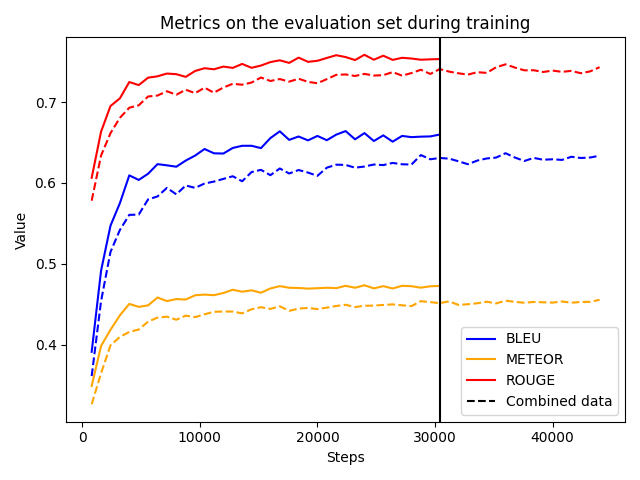
\includegraphics[width=0.60\textwidth]{Images/jointGT_training.png}
%    \caption{Computed metrics per evaluation (each 800 steps). Vertical line indicates stop of training on the non-combined dataset}
%    \label{fig:training_jointgt}
%\end{figure}

\begin{table}[ht]
\caption{The performance metrics of the best performing model on their corresponding validation and test set -- either WebNLG or the combined set. Both models are evaluated also on the FARO test set}
\centering
\begin{tabular}{|l|l|l|l|l|l|l|}
\hline
\textbf{Model}                 & \textbf{Dataset} & \textbf{BLEU} & \textbf{METEOR} & \textbf{ROUGE} & \textbf{Step} & \textbf{Epoch} \\ \hline
\multirow{3}{*}{Base (WebNLG)} & Val              & 0.6642        & 0.4727          & 0.7558         & 22400         & 6              \\ \cline{2-7} 
                               & Test             & 0.6529        & 0.4681          & 0.7535         & -             & -              \\ \cline{2-7} 
                               & FARO test        & 0.0           & 0.0565           & 0.1299         & -             & -              \\ \hline
\multirow{3}{*}{Combined}      & Val              & 0.6368        & 0.4543          & 0.7468         & 36000         & 9              \\ \cline{2-7} 
                               & Test             & 0.6101        & 0.4409          & 0.7260         & -             & -              \\ \cline{2-7} 
                               & FARO test        & 0.0477        & 0.0877          & 0.1949         & -             & -              \\ \hline
\end{tabular}

\label{tab:training_jointgt}
\end{table}

%Figure~\ref{fig:training_jointgt} reports the BLEU, METEOR and ROUGE scores on the evaluation set during training.\footnote{The model stops training if no improvement has been made in 10 evaluations} Together with Table \ref{tab:training_jointgt}, it reveals important insights into the model's performance. The ROUGE metric indicates a relatively high level of performance, suggesting that the model generates text that closely aligns with the reference texts in terms of information. In contrast, the BLEU metric exhibits slightly lower performance, implying that the model's output words differ slightly from those in the reference texts. The relatively low METEOR score could be attributed to how the predicted and reference texts are aligned when calculating the score. It is worth noting that the base model's performance on the test set aligns closely with the results reported in the original JointGT paper~\cite{JointGT}.
Table \ref{tab:training_jointgt} provides crucial insights into the model's performance. ROUGE suggests a high level of alignment with reference texts in conveying information, while BLEU shows minor word deviations from references. The lower METEOR score might stem from alignment nuances in score calculation. Notably, the base model's test performance closely mirrors the results outlined in the original JointGT paper~\cite{JointGT}.
The model that was trained on the combined dataset performed slightly worse for all three metrics than the model that was trained on the base WebNLG data. This can be explained by two considerations. First, it is evident in Table \ref{tab:training_jointgt} that tests on FARO have very low performances. Secondly, the FARO dataset only accounts for a relatively small proportion in the combined dataset (Table \ref{tab:splits_dataset_jointgt}). To better understand the reasons, a qualitative analysis is proposed in the next section.

\subsection{Qualitative analysis.}
\begin{sidewaystable}[ph!]
\caption{Sample of the FARO test-set and the generated output of the base- and combined model}
\resizebox{\textwidth}{!}{  
\begin{tabular}{|l|l|l|l|}
\hline
\textbf{Triple}          & \textbf{Label}                                                                                                                                                                                                               & \textbf{Base generated}                                                            & \textbf{Combined generated}                                                                                                                                                                                       \\ \hline
(offer, cause, reimburse) & \begin{tabular}[c]{@{}l@{}}(The directors said if Messrs. Drabinsky\\ and Gottlieb mail an offer to shareholders by\\ Nov. 22, it will reimburse them a maximum\\ of C\$8.5 million for expenses related to a bid.)\end{tabular} & \begin{tabular}[c]{@{}l@{}}The cause of the offer is to\\ reimburse .\end{tabular} & \begin{tabular}[c]{@{}l@{}}The company has also announced\\ that it will offer a new credit\\ facility to small businesses, in an\\ effort to reimburse them for the cost\\ of capital expenditures.\end{tabular} \\ \hline
\end{tabular}
}

\label{tab:combined_base_farotest-set}

\resizebox{\textwidth}{!}{
\begin{tabular}{|l|l|l|}
\hline
\textbf{Triple}                                                                                                                                                                                  & \textbf{Label}                                                                                                                                                                                                                                                                                              & \textbf{Generated}                                                                                                                                   \\ \hline
\begin{tabular}[c]{@{}l@{}}(3Arena, owner, Live Nation\\ Entertainment), (Dublin, is part\\ of, Republic of Ireland),\\ (3Arena, location, Dublin),\\ (Dublin, is part of, Leinster)\end{tabular} & \begin{tabular}[c]{@{}l@{}}(The owner of 3Arena , Dublin , Leinster , Republic\\ of Ireland is Live Nation Entertainment .), (Dublin\\ is part of Leinster and a city in the Republic of\\ Ireland . Dublin is also home to the 3Arena which\\ is currently owned byLive Nation Entertainment.)\end{tabular} & \begin{tabular}[c]{@{}l@{}}3Arena is located in Dublin , Leinster ,\\ Republic of Ireland and is owned by\\ Live Nation Entertainment .\end{tabular} \\ \hline
\end{tabular}
}
\caption{Sample of the WebNLG test-set and the generated output of the base model.}
\label{tab:base_WebNLGtest-set}
\end{sidewaystable}

We examine instances from WebNLG and FARO datasets to analyze the base and combined model's performance. Observing Tables \ref{tab:combined_base_farotest-set} and \ref{tab:base_WebNLGtest-set}, the text generated by the combined dataset-trained model appears more semantically robust. The base model's generated text for FARO triples (Table \ref{tab:combined_base_farotest-set}, column \textit{Base generated}) is notably brief, often mirroring the triples with semantic inaccuracies. Conversely, the combined model produces more coherent and accurate sentences in the same dataset (column \textit{Combined generated}), maintaining triple direction. However, it's important to note that while the generated content respects triple order and semantic accuracy, it may still have limitations in altering the original label's content.
% The other sentences are correct, while also incorporating the subject and object of the triple and making the sentence of the same correct relation type. But since there is only 1 triple per sentence, the model has to generate a lot of words to create a valid sentence. Looking at the other table where the base model is tested on the WebNLG data, where there are multiple input triples per instance, it can be seen that for all the instances, the model is able to incorporate those triples and generating a semantically correct sentence in all 5 cases.

We also get a sight why the quantitative results are slightly worst for the combined model. The WebNLG data (Table \ref{tab:base_WebNLGtest-set}) contains multiple triples per instance, giving more information about the text, and contains multiple labels. The FARO data (Table \ref{tab:combined_base_farotest-set}) contains only one triple per instance, together with one target sentence (label). Therefore, the model has less information about what to generate, and less chances to match the target label. Looking at the FARO input triples and the target label, it can be seen that the relationship (predicate) is often not explicitly represented by a particular word in the target sentence (implicit relation), making the evaluation with matching words harder. We provide additional insights in Appendix \ref{sec:appendix}.

\paragraph*{User Evaluation on ASRAEL}
\label{sec:result_gen_text_nodes}
To evaluate the system's performance, seven events from the ASRAEL dataset have been selected based on several criteria: values for the 4W properties, a minimal number of articles, etc. The two largest events from this group are selected for evaluation: \textit{``Operation Breaking Dawn"}, and \textit{``2021 storming of the United States Capitol"}. Among the remaining events that include information about the place and time, five additional events are selected.
% \begin{itemize}
%     \item Operation Breaking Dawn (where, when, who, mentions)
%     \item 2021 storming of the United States Capitol (where, when, who, mentions)
%     \item 2021 Fukushima earthquake (where, when, mentions)
%     \item 2021 Sundance Film Festival (where, when, mentions)
%     \item Giza church fire (where, when, mentions)
%     \item Nationwide COVID-19 memorial (where, when, mentions)
%     \item Save America March (where, when, mentions)
% \end{itemize}

The information selection method is used to select time, place, actor, and up to three mentions from the seven selected events. The base and combined models are used to generate text from the selected information. This information per event can be found in Appendix \ref{sec:appendix}, together with the generated text. Manual evaluation needed due to no reference text for automated metrics.

Three annotators per event determined the superior text between two models, by using either: ``win", ``lose", or ``tie". Assessing "fluency" (grammatical correctness) and "adequacy" (correct integration of triples). This method aligns with the approach in \cite{JointGT}. Majority voting determined the winner or equality between models, followed by a non-parametric "sign test" at a significance level of $\alpha$ = 0.05 to establish superiority. Results of this annotation are accessible in Table \ref{tab:event_annotations}.

The combined model produces better fluent text than the base model in 71.4\% of the cases. The non-parametric ``signed test" was performed to measure a significant difference in the fluency of the text. With a p-value of 0.11, no significant difference was found. The same was done to gauge the text's adequacy. With a p-value of 0.25, no significant difference was found.

\begin{table}[ht]
\caption{Fleiss' Kappa ($\kappa$) indicates perfect, and moderate agreement between annotators. The wins, losses, and ties when comparing the combined model against the base model are indicated in percentages. No model was significantly better than another with a significance level of 0.05.}

\centering
\begin{tabular}{|c|lll|l|lll|l|}
\hline
\multirow{2}{*}{Model}                 & \multicolumn{3}{c|}{Fluency}                                     & \multirow{2}{*}{$\kappa$} & \multicolumn{3}{c|}{Adequacy}                                    & \multirow{2}{*}{$\kappa$} \\ \cline{2-4} \cline{6-8}
                                       & \multicolumn{1}{l|}{Win \%} & \multicolumn{1}{l|}{Lose \%} & Tie \% &                    & \multicolumn{1}{l|}{Win \%} & \multicolumn{1}{l|}{Lose \%} & Tie \% &                    \\ \hline
\multicolumn{1}{|l|}{Combined vs Base} & \multicolumn{1}{l|}{71.4}  & \multicolumn{1}{l|}{14.3}   & 14.3  & 1.0                & \multicolumn{1}{l|}{28.6}  & \multicolumn{1}{l|}{0.0}    & 71.4  & 0.6                \\ \hline
\end{tabular}
\label{tab:event_annotations}
\end{table}

\paragraph*{User Evaluation on an Manually Annotated Event} 
\label{sec:result_gen_event}

To demonstrate whether the obtained results are consistent independently from the quality of the information extraction output, we decided to perform a user evaluation on a single article (sample), which has been manually annotated by users, which handcrafted the resulting subgraph. This subgraph has been processed with both the combined and base model, and then evaluated using either ``win", ``lose", or ``tie", in the same way as described in the previous section. The percentage of wins, losses and ties for the combined model, together with the Fleiss' kappa are reported in Table \ref{tab:article_annotations}. The combined model has been assigned more wins for producing fluent and adequate text. The non-parametric ``signed test" is applied to test if this is significant, again, with a significance level of 0.05. With a p-value of 0.34, no significant difference is found in generating more fluent texts between models. With a p-value of 0.04, a significant difference is found in generating more adequate sentences by the combined model, compared to the base model.

\begin{table}[ht]
\caption{Fleiss' Kappa ($\kappa$) indicates substantial agreement between annotators. The wins, losses, and ties when comparing the combined model against the base model are indicated in percentages. The combined model was significantly better than the base model in generating adequate sentences.}

\centering
\begin{tabular}{|c|lll|l|lll|l|}
\hline
\multirow{2}{*}{Model}                 & \multicolumn{3}{c|}{Fluency}                                        & \multirow{2}{*}{$\kappa$} & \multicolumn{3}{c|}{Adequacy}                                       & \multirow{2}{*}{$\kappa$} \\ \cline{2-4} \cline{6-8}
                                       & \multicolumn{1}{l|}{Win \%} & \multicolumn{1}{l|}{Lose \%} & Tie \% &                    & \multicolumn{1}{l|}{Win \%} & \multicolumn{1}{l|}{Lose \%} & Tie \% &                    \\ \hline
\multicolumn{1}{|l|}{Combined vs Base} & \multicolumn{1}{l|}{33.3}   & \multicolumn{1}{l|}{16.7}    & 50.0   & 0.73               & \multicolumn{1}{l|}{58.3}   & \multicolumn{1}{l|}{8.3}     & 33.3   & 0.61               \\ \hline
\end{tabular}
\label{tab:article_annotations}
\end{table}

BLEU, METEOR, and ROUGE metrics have been computed using the sentences from the article as ``reference label". These scores are detailed in Table \ref{tab:article_auto_metrics}. This illustrates that the base model performs slightly better than the model that was trained on the combined data. A reason for this could be formulated by looking at the generated texts, which can be found in Appendix. The base model will, more often than the combined model, output parts of the triple without taking the relationship between them into account. This will result in a badly formed sentence, but higher metrics, since more triples are incorporated. This is also reflected in the scores in Table \ref{tab:article_annotations}, Where the combined model is commonly noted for producing more fluent texts.

Table \ref{tab:article_auto_metrics} shows the metric scores for the article. These scores are much lower then those computed on the WebNLG test (Table \ref{tab:training_jointgt}). This outcome could be expected, considering that some of the triples extracted from the article are not, or to a limited extend, present in the original WebNLG data used to pre-train the JointGT model.

\begin{table}[]
\caption{BLEU, METEOR, and ROUGE scores per model on the generated text from the article}
\centering
\begin{tabular}{|l|l|l|l|}
\hline
\textbf{Model} & \textbf{BLEU} & \textbf{METEOR} & \textbf{ROUGE} \\ \hline
Combined       & 0.1681        & 0.2081          & 0.3622         \\ \hline
Base           & 0.1874        & 0.2273          & 0.3738         \\ \hline
\end{tabular}

\label{tab:article_auto_metrics}
\end{table}

\section{Conclusion and Future Work}
\label{sec:conclusion}
The primary goal of this research is to investigate how to build complex narratives in the form of graphs of events, generating text with good level of complexity and semantic richness, expecting the system to generate answers beyond only  
 \textit{What} (event), \textit{Who} (actor), \textit{Where} (location), and \textit{When} (time).

% We enhanced the WebNLG dataset with the FARO dataset, for improving the semantic quality of event relations. This enrichment introduced complexity to the dataset by incorporating event relations such as causality, prevention, intention, and enabling. We applied state-of-art methods to extract semantically precise relations from news articles and to perform event co-reference resolution, to generate a so-called \textit{narrative graph}. We use a heuristic to select the most important nodes, which we feed to JointGT to generate natural text. Given accurate extraction of sub-events and relations, this setup represents a promising approach for generating natural text that incorporates information from the constructed narrative graph. The full code and experiments are available at \url{https://anonymous.4open.science/r/KG2Narrative}.
%\url{https://github.com/ANR-kFLOW/KG2Narrative}.
We enhanced the WebNLG dataset through the incorporation of the FARO dataset, aimed at refining the semantic depth of event relations. The expanded dataset now encompasses intricate relations including causality, prevention, intention, and enabling. 
From qualitative analysis, we can state that training on precise event relations produces more complete generated sentences, while no statistically significant difference was observed on fluency. Future work will experiment on more data to draw final conclusions. 
% However, we also observe some limitations. Events and relations are extracted from each sentence in an article, which can result in incorrect extractions since not every sentence may contain these elements. The selection of information from the graph is limited to the primary event of interest, neglecting relevant information from other connected events. The data used for fine-tuning was different from the original dataset in terms of triple counts and instances, potentially affecting model evaluation. Furthermore, it is worth highlighting that the content generated, while maintaining triple order and semantic accuracy, has sometimes constraints in terms of altering the original label's content. Future work may involve selectively extracting sub-events and relations at the document level to improve clustering. Lastly, acquiring additional data using NLP techniques is suggested to enhance the dataset.
Our information selection from the graph focuses solely on the main event, disregarding pertinent details from interconnected events. Additionally, the data used for fine-tuning differs from the original dataset in terms of triple counts and instances, potentially impacting model evaluation. Future research could explore selectively extracting sub-events and relations at the document level to enhance clustering. Moreover, augmenting the dataset through NLP techniques could significantly improve its quality and comprehensiveness.






% \section*{Acknowledgements}
% This work has been partially supported by the French National Research Agency (ANR) within the kFLOW project (Grant n°ANR-21-CE23-0028).

\bibliography{bibliography}




\pagebreak


\appendix

\section{Appendix}
\label{sec:appendix}

\subsection{Results REBEL Model}
\begin{table}[!h]
\centering
\begin{tabular}{|l|l|l|l|l|l|l|}
\hline
\textbf{Relation} & \textbf{Precision} & \textbf{Recall} & \textbf{F1} & \textbf{Support} & \textbf{Micro F1}      & \textbf{Macro F1}      \\ \hline
Cause             & 80.00              & 96.00           & 87.27       & 25               & \multirow{4}{*}{94.03} & \multirow{4}{*}{93.13} \\ \cline{1-5}
Enable            & 94.55              & 94.55           & 94.55       & 55               &                        &                        \\ \cline{1-5}
Prevent           & 98.21              & 91.67           & 94.83       & 60               &                        &                        \\ \cline{1-5}
Intend            & 96.67              & 95.08           & 95.87       & 61               &                        &                        \\ \hline
\end{tabular}
\caption{Detailed result for the validation dataset using the REBEL model}
\label{apx:val_result_rebel}
\end{table}

\begin{table}[!h]
\centering
\begin{tabular}{|l|l|l|l|l|c|l|}
\hline
\textbf{Relation} & \textbf{Precision} & \textbf{Recall} & \textbf{F1} & \textbf{Support} & \multicolumn{1}{l|}{\textbf{Micro F1}} & \textbf{Macro F1}      \\ \hline
Cause             & 85.19              & 100.00          & 92.00       & 46               & \multirow{4}{*}{85.71}                 & \multirow{4}{*}{82.12} \\ \cline{1-5}
Enable            & 84.62              & 61.11           & 70.97       & 18               &                                        &                        \\ \cline{1-5}
Prevent           & 84.62              & 68.75           & 75.86       & 16               &                                        &                        \\ \cline{1-5}
Intend            & 92.86              & 86.67           & 89.66       & 15               &                                        &                        \\ \hline
\end{tabular}
\caption{Detailed result for the test dataset using the REBEL model}
\label{apx:test_result_rebel}
\end{table}

%Maybe break this images up, if it is not readable
\begin{figure}[!h]
    \centering
    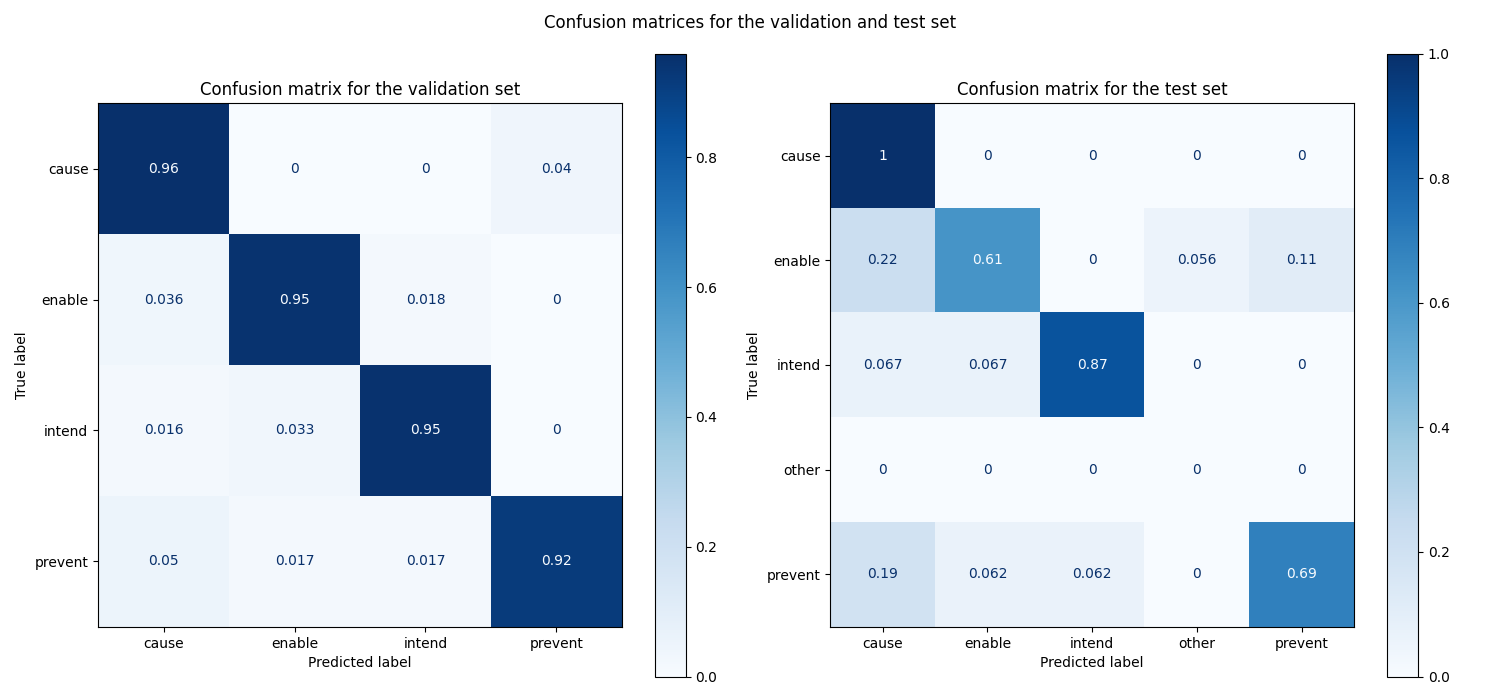
\includegraphics[width=1.2\textwidth]{Images/Confusion_matrix.png}
    \caption{Confusion matrix of relationships in the validation- and testset}
    \label{fig:confusion_matrix}
\end{figure}

\begin{table}[!h]
\centering
\begin{tabular}{|l|l|}
\hline
\textbf{Relation}    & \textbf{Frequency} \\ \hline
has cause            & 1584               \\ \hline
cause of destruction & 55                 \\ \hline
has immediate cause  & 14                 \\ \hline
immediate cause of   & 9                  \\ \hline
end cause            & 3                  \\ \hline
may prevent          & 2                  \\ \hline
\end{tabular}
\caption{Relationships in the REBEL train dataset}
\label{apx:rebel_rel}
\end{table}

\subsection{Event coreference resolution}

\begin{figure}[!h]
    \centering
    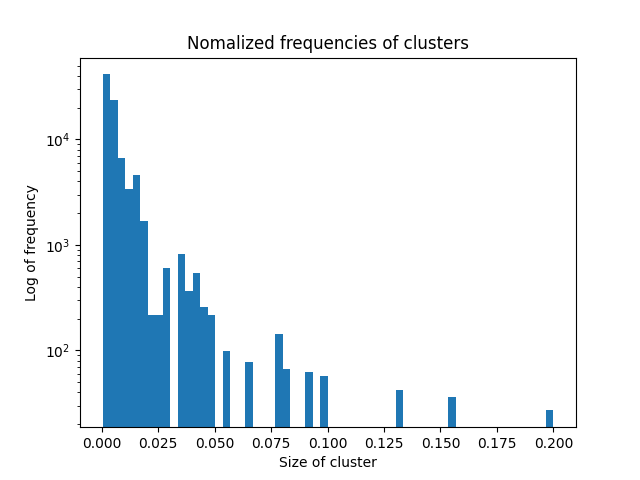
\includegraphics[scale=0.5]{Images/norm_freq_cluster_size.png}
    \caption{Normalized distribution of the cluster sizes}
    \label{fig:norm_freq_cluster_size}
\end{figure}

\subsection{JointGT: Qualitative analysis}
\begin{sidewaystable}[]
\begin{tabular}{|l|l|l|}
\hline
\textbf{Triples}                                                                                                                                                                                                        & \textbf{Label}                                                                                                                                                                                                                                                                                                                                                                                                                                                                                       & \textbf{Generated}                                                                                                                                                                 \\ \hline
\begin{tabular}[c]{@{}l@{}}(109 Felicitas, apoapsis, 523329000.0 (kilometres),\\ (109 Felicitas, temperature, 170.0 (kelvins))\end{tabular}                                                                             & \begin{tabular}[c]{@{}l@{}}(109 Felicitas , with a temperature of 170 kelvins , \\ has an apoapsis of 523329000.0 ( kilometres ) .), \\ (The temperature of the asteroid called 109 Felicitas is\\  170.0 kelvins and it has an apoapsis of 523329000.0 km .),\\ (The temperature of the asteroid called 109\\ Felicitas is 170.0 kelvins and it has an apoapsis of\\ 523329000 kilometres .)\end{tabular}                                                                                           & \begin{tabular}[c]{@{}l@{}}109 Felicitas has an apoapsis of 523329000.0\\ kilometres and a temperature of 170.0 kelvins .\end{tabular}                                             \\ \hline
\begin{tabular}[c]{@{}l@{}}(3Arena, owner, Live Nation Entertainment),\\ (Dublin, is part of, Republic of Ireland),\\ (3Arena, location, Dublin),\\ (Dublin, is part of, Leinster)\end{tabular}                         & \begin{tabular}[c]{@{}l@{}}(The owner of 3Arena , Dublin , Leinster , \\ Republic of Ireland is Live Nation Entertainment .),\\ (Dublin is part of Leinster and a city in the Republic\\ of Ireland .Dublin is also home to the 3Arena which is\\ currently owned by Live Nation Entertainment .)\end{tabular}                                                                                                                                                                                       & \begin{tabular}[c]{@{}l@{}}3Arena is located in Dublin , Leinster , \\ Republic of Ireland and is owned by\\ Live Nation Entertainment .\end{tabular}                              \\ \hline
(Barny Cakes, serving size, 30.0 g)                                                                                                                                                                                     & \begin{tabular}[c]{@{}l@{}}(Barny cakes can be served in 30 gram sizes .),\\ (Serving size for the Barny cakes is 30.0g .),\\ (The serving size of Barny cakes is 30.0g .)\end{tabular}                                                                                                                                                                                                                                                                                                              & Barny cakes have a serving size of 30.0 g .                                                                                                                                        \\ \hline
\begin{tabular}[c]{@{}l@{}}(107 Camilla, discoverer, N.R. Pogson), \\ (N. R. Pogson, death place, Chennai),\\ (107 Camilla, periapsis, 479343000.0 (kilometres),\\ (N. R. Pogson, birth place, Nottingham)\end{tabular} & \begin{tabular}[c]{@{}l@{}}(Nottingham born , N.R . Pogson ( who died in Chennai ) ,\\ discovered 107 Camilla , which has a periapsis of\\ 479343000.0kilometres .), (N.R . Pogson discovered 107\\ Camilla which has a periapsis of 479,343,000 kilometres .\\ Pogson was born in Nottingham and died in Chennai .),\\ (107 Camilla was discovered by N.R . Pogson who was born\\ in Nottingham . He died in Chennai . The periapsis of 107\\ Camilla is 479343000.0 ( kilometres ) .)\end{tabular} & \begin{tabular}[c]{@{}l@{}}N.R . Pogson was born in Nottingham and\\ died in Chennai . He discovered 107 Camilla\\ which has a periapsis of479343000.0\\ kilometres .\end{tabular} \\ \hline
('Fulton County, Georgia', country, United States)                                                                                                                                                                      & \begin{tabular}[c]{@{}l@{}}(Fulton County is in Georgia , in the United States .),\\ (Fulton County , in Georgia is part of the U.S .)\end{tabular}                                                                                                                                                                                                                                                                                                                                                  & Fulton County , Georgia is in the United States .                                                                                                                                  \\ \hline
\end{tabular}
\caption{Sample of the WebNLG testset and the generated output of the base model.}
\label{tab:base_webnlgTestset}
\end{sidewaystable}


\clearpage
\begin{sidewaystable}[]
\begin{tabular}{|l|l|l|}
\hline
\textbf{Triples}                & \textbf{Labels}                                                                                                                                                                                                                                                                  & \textbf{Generated}                        \\ \hline
(demand, cause, benefited)      & \begin{tabular}[c]{@{}l@{}}(The company benefited from continued\\ strong demand and higher selling prices\\ for titanium dioxide, a white pigment used\\ in paints, paper and plastics.)\end{tabular}                                                                           & benefited '' is the cause of the demand . \\ \hline
(center, enable, innovation)    & \begin{tabular}[c]{@{}l@{}}(We recently moved our headquarters and\\ research and development center to\\ Abu Dhabi to benefit from its rapidly\\ growing innovation hub, and with the new\\ AWS Region, we are excited to see it thrive\\ at an accelerated rate.)\end{tabular} & Innovation is the enabler of the center . \\ \hline
(made, cause, eaten)            & \begin{tabular}[c]{@{}l@{}}("Cheerios and Honey Nut Cheerios have\\ eaten away sales normally going to Kellogg\'s\\ corn-based lines simply because they are\\ made of oats," says Merrill Lynch food\\ analyst William Maguire.)\end{tabular}                                   & The cause of eating is eaten .            \\ \hline
(offer, cause, reimburse)       & \begin{tabular}[c]{@{}l@{}}(The directors said if Messrs. Drabinsky\\ and Gottlieb mail an offer to shareholders by\\ Nov. 22, it will reimburse them a maximum\\ of C\$8.5 million for expenses related to a bid.)\end{tabular}                                                  & The cause of the offer is to reimburse .  \\ \hline
(proclaimed, prevent, bloodhed) & \begin{tabular}[c]{@{}l@{}}(DR Congo President Felix Tshisekedi on\\ May 6 proclaimed a 30-day "state of siege"\\ -- effectively martial law -- in North Kivu\\ and neighbouring Ituri province in a bid to\\ curb bloodshed by the ADF.)\end{tabular}                           & Bloodshed can be prevented .              \\ \hline
\end{tabular}
\caption{Sample of the FARO testset and the generated output of the base model}
\label{tab:base_faroTestset}
\end{sidewaystable}


\clearpage
\begin{sidewaystable}[]
\begin{tabular}{|l|l|l|}
\hline
\textbf{Triples}                & \textbf{Labels}                                                                                                                                                                                                                                                                  & \textbf{Generated}                                                                                                                                                                                            \\ \hline
(demand, cause, benefited)      & \begin{tabular}[c]{@{}l@{}}(The company benefited from continued\\ strong demand and higher selling prices\\ for titanium dioxide, a white pigment used\\ in paints, paper and plastics.)\end{tabular}                                                                           & \begin{tabular}[c]{@{}l@{}}The company said it benefited from the strong demand\\ for its products and services from a growing number of customers.\end{tabular}                                              \\ \hline
(center, enable, innovation)    & \begin{tabular}[c]{@{}l@{}}(We recently moved our headquarters and\\ research and development center to\\ Abu Dhabi to benefit from its rapidly\\ growing innovation hub, and with the new\\ AWS Region, we are excited to see it thrive\\ at an accelerated rate.)\end{tabular} & \begin{tabular}[c]{@{}l@{}}The United States has created a new innovation center that\\ will help stimulate economic growth and job creation.\end{tabular}                                                    \\ \hline
(made, cause, eaten)            & \begin{tabular}[c]{@{}l@{}}("Cheerios and Honey Nut Cheerios have\\ eaten away sales normally going to Kellogg\'s\\ corn-based lines simply because they are\\ made of oats," says Merrill Lynch food\\ analyst William Maguire.)\end{tabular}                                   & \begin{tabular}[c]{@{}l@{}}The company said it made a profit from the sale of the shares\\ because it made enough money to make a profit from the sale.\end{tabular}                                          \\ \hline
(offer, cause, reimburse)       & \begin{tabular}[c]{@{}l@{}}(The directors said if Messrs. Drabinsky\\ and Gottlieb mail an offer to shareholders by\\ Nov. 22, it will reimburse them a maximum\\ of C\$8.5 million for expenses related to a bid.)\end{tabular}                                                  & \begin{tabular}[c]{@{}l@{}}The company has also announced that it will offer a new credit\\ facility to small businesses, in an effort to reimburse them\\ for the cost of capital expenditures.\end{tabular} \\ \hline
(proclaimed, prevent, bloodhed) & \begin{tabular}[c]{@{}l@{}}(DR Congo President Felix Tshisekedi on\\ May 6 proclaimed a 30-day "state of siege"\\ -- effectively martial law -- in North Kivu\\ and neighbouring Ituri province in a bid to\\ curb bloodshed by the ADF.)\end{tabular}                           & \begin{tabular}[c]{@{}l@{}}The United Nations has proclaimed a new resolution to\\ prevent the spread of bloodshed.\end{tabular}                                                                              \\ \hline
\end{tabular}
\caption{Sample of the FARO testset and the generated output of the combined model}
\label{tab:combined_faroTestset}
\end{sidewaystable}
\clearpage

\subsection{Generating text from selected events}
\label{appx:selected_processed_events}

\textbf{Operation Breaking Dawn}
\begin{itemize}
    \item begin date: 2022-08-05
    \item end date: 2021-08-07
    \item location: Israel
    \item participant: Israel Defense Forces
    \item triples: $<bombardment,\;cause,\;firing>,\; <bombardment,\; cause,\; retaliated>,\; <fired,\; cause,\; killed>$
\end{itemize}
Base model: \textit{"Israel Defense Forces participated in Operation Breaking Dawn which began on August 5th, 2022 and ended on July 7th, 2022. The bombardment was retaliated by firing."}\\\\
\noindent
Combined model: \textit{"Israel Defense Forces participated in Operation Breaking Dawn which began on August 5th, 2022 and ended on July 7th, 2022. The Israelis were involved in Operation Breaking Dawn and were killed in the retaliation of the Israelis."}\\\\
\noindent

\textbf{2021 storming of the United States Capitol}
\begin{itemize}
    \item date: 2021-01-06
    \item location: United States of America
    \item participant: Proud Boys
    \item triples: $<measures,\;enable,\;removing>,\; <died,\; cause,\; shot>,\; <addressed,\; cause,\; shot>$
\end{itemize}
Base model: \textit{"Save America March is located in the United States of America and was launched on January 6th, 2021. Its cause was stormed and it was removed."}\\\\
\noindent
Combined model: \textit{"Save America March is located in the United States of America and was launched on January 6th, 2021. The US government has implemented a series of measures to prevent the spread of disasters."}\\\\
\noindent

\textbf{2021 Fukushima earthquake}
\begin{itemize}
    \item: date: 2021-02-13
    \item location: Japan
    \item triples: $<earthquake,\;cause,\;collapsing>,\; <earthquake,\; cause,\; injured>,\; <broken,\; cause,\; damage>$
\end{itemize}
Base model: \textit{"2021 Fukushima earthquake, which was caused by collapsing, is located in Japan and was broken."}\\\\
\noindent
Combined model: \textit{"The 2021 Fukushima earthquake, which hit Japan on February 13th, 2021, injured many people and caused extensive damage and collapsing."}\\\\
\noindent

\textbf{2021 Sundance Film Festival}
\begin{itemize}
    \item begin date: 2021-01-28
    \item end date: 2021-02-03
    \item location United States of America
    \item triples: $<whittled,\;cause,\;unveiling>,\; <awards,\; enable,\; stunt>,\; <coronavirus pandemic,\; cause,\; delayed>$
\end{itemize}
Base model: \textit{"2021 Sundance Film Festival, located in the United States of America, began on January 28th, 2021 and ended on March 3rd, 2021-02-03. The event was delayed by the coronavirus pandemic, and awards were whittled."}\\\\
\noindent
Combined model: \textit{"2021 Sundance Film Festival, which is located in the United States, began on January 28th, 2021 and ended on March 3rd, 2021. It was delayed because of the coronavirus pandemic."}\\\\
\noindent

\textbf{Giza church fire}
\begin{itemize}
    \item date: 2022-08-14
    \item location: Egypt
    \item triples: $<mobilized,\;cause,\;taken>,\; <went,\; cause,\; deaths>,\; <short circuit,\; cause,\; fire>$
\end{itemize}
Base model: \textit{"The cause of the Giza church fire, which was located in Egypt, was a short circuit. The church was mobilised on the 14th of August, 2022."}\\\\
\noindent
Combined model: \textit{"The Giza church fire, which occurred on 2022-08-14, was located in Egypt. It was a short circuit that killed several people."}\\\\
\noindent

\textbf{Nationwide COVID-19 memorial}
\begin{itemize}
    \item date: 2021-01-19
    \item location: United States of America
    \item triples: $<pandemic,\;prevent,\;swearing-in>,\; <confirmation,\; cause,\; run>,\; <sworn,\; cause,\; saluted>$
\end{itemize}
Base model: \textit{"The nationwide COVID-19 Memorial, located in the United States of America, was sworn in on January 19th, 2021. It was saluted and run to prevent a pandemic."}\\\\
\noindent
Combined model: \textit{"The National COVID-19 Memorial is located in the United States of America and was inaugurated 
on January 19th, 2021. It was saluted and sworn in to prevent a pandemic."}\\\\
\noindent

\textbf{Save America March}
\begin{itemize}
    \item date: 2021-01-06
    \item location: United States of America
    \item triples: $<measures,\;enable,\;removing>,\; <emergencies,\; cause,\; died>,\; <stormed,\; cause,\; drew>$
\end{itemize}
Base model: \textit{"Save America March is located in the United States of America and was launched on January 6th, 2021. Its cause was stormed and it was removed."}\\\\
\noindent
Combined model: \textit{"Save America March is located in the United States of America and was launched on January 6th, 2021. The US government has implemented a series of measures to prevent the spread of disasters."}



\subsection{Annotation of article: Russia launches Iranian satellite amid Ukraine war concerns}
\label{appx:article_annotation}

\textbf{An Iranian satellite launched by Russia blasted off from Kazakhstan Tuesday and reached orbit amid controversy that Moscow might use it to boost its surveillance of military targets in Ukraine}\\\\
\noindent
Triples: ("Russia", "launch", "satellite"), ("launch", "location", "Kazakhstan"), ("launch", "time", "Tuesday"), ("satellite", "enable", "military surveillance")\\\\
\noindent
Base model: \textit{"The launch of a satellite in Kazakhstan , which has a military surveillance capability , took place on Tuesday ."}\\\\
\noindent
Combined model: \textit{"The launch of a satellite from Russia was on Tuesday , in Kazakhstan . The satellite will enable military surveillance of the country ."}\\\\\\\\
\noindent
\textbf{As Russia's international isolation grows following Western sanctions over its invasion of Ukraine, the Kremlin is seeking to pivot towards the Middle East, Asia and Africa and find new clients for its embattled space programme.}\\\\
\noindent
Triples: ("Russia", "cause", "invasion of Ukraine"), ("invasion of Ukraine", "cause", "western sanctions"), ("western sanctions", "cause", "Russia's international isolation"), ("Russia", "intend", "find new clients")\\\\
\noindent
Base model: \textit{"Russia 's invasion of Ukraine is caused by western sanctions and Russia 's international isolation . Russia 's intention is to find new clients ."}\\\\
\noindent
Combined model: \textit{"The invasion of Ukraine is a cause of Russia 's isolation and western sanctions are a reason for Russia's invasion of Ukraine . Russia also seeks to find new clients in the region ."}\\\\\\
\noindent
\textbf{Speaking at the Moscow-controlled Baikonur Cosmodrome in the Kazakh steppe, Russian space chief Yury Borisov hailed "an important milestone in Russian-Iranian bilateral cooperation, opening the way to the implementation of new and even larger projects".}\\\\
\noindent
Triples: ("Russian-Iranian bilateral cooperation", "enable", "implementation of new and even larger projects")\\\\
\noindent
Base model: \textit{"The Russian-Iranian bilateral cooperation is enabled by the implementation of new and even larger projects ."}\\\\
\noindent
Combined model: \textit{"The Russian-Iranian bilateral cooperation will enable the implementation of new and even larger projects ."}\\\\\\
\noindent
\textbf{Iran's Telecommunications Minister Issa Zarepour, who also attended the launch of the Khayyam satellite, called the event "historic" and "a turning point for the start of a new interaction in the field of space between our two countries".}\\\\
\noindent
Triples: ("Iran Telecommunication", "minister", "Issa Zarepour"), ("Issa Zarepour", "attended", "launch of the Khayyam satellite"), ("satellite", "enable", "a turning point for the start of a new interaction")\\\\
\noindent
Base model: \textit{"Iran Telecommunications Minister Issa Zarepour attended the launch of the Khayyam satellite , which was a turning point for the start of a new interaction ."}\\\\
\noindent
Combined model: \textit{"Iran Telecommunication Minister Issa Zarepour attended the launch of the Khayyam satellite , which was a turning point for the start of a new interaction ."}\\\\\\
\noindent
\textbf{Nasser Kanani, the Iranian foreign ministry spokesman, said on Twitter that "the brilliant path of scientific and technological progress of the Islamic republic of Iran continues despite sanctions and the enemies' maximum pressure".}\\\\
\noindent
Triples: ("western sanctions", "not prevent", "scientific and technological progress of Iran"), ("enemies' maximum pressure", "not prevent", "scientific and technological progress of Iran")\\\\
\noindent
Base model: \textit{"The enemies ' maximum pressure is the scientific and technological progress of Iran ."}\\\\
\noindent
Combined model: \textit{"The United Nations has imposed a maximum pressure on Iran in an effort to prevent the country from achieving scientific and technological progress."}\\\\\\
\noindent
\textbf{Iran, which has maintained ties with Moscow and refrained from criticism of the Ukraine invasion, has sought to deflect suspicions that Moscow could use Khayyam to spy on Ukraine.}\\\\
\noindent
Triples: ("Iran", "maintained ties", "Moscow", 5), ("Iran", "not criticized", "Ukraine invasion", 5), ("Khayyam", "enable", "spy", 5)\\\\
\noindent
Base model: \textit{"Khayyam is a spy in Iran , which has maintained ties with Moscow . The Ukraine invasion is not criticized in Iran ."}\\\\
\noindent
Combined model: \textit{"Khayyam was allowed to spy on Moscow and Iran , which has not been criticized for its invasion of Ukraine ."}\\\\\\
\noindent
\textbf{Responding to the launch, Washington said Russia's growing cooperation with Iran should be viewed as a "profound threat".}\\\\
\noindent
Triples: ("Washington", "respond", "launch"), ("Russia's growing cooperation with Iran", "cause", "profound threat")\\\\
\noindent
Base model: \textit{"Russia 's growing cooperation with Iran is the cause of Washington 's response , which is a profound threat ."}\\\\
\noindent
Combined model: \textit{"Russia's growing cooperation with Iran has created a profound threat to the region, and the United States has responded with a missile launch."}\\\\\\
\noindent
\textbf{"No third country is able to access the information" sent by the satellite due to its "encrypted algorithm", it said.}\\\\
\noindent
Triples: ("satellite", "sends", "information"), ("encrypted algorithm", "prevent", "third countries accessing information"), ("satellite", "has", "encrypted algorithm")\\\\
\noindent
Base model: \textit{"The satellite has an encrypted algorithm which prevents third countries accessing information ."}\\\\
\noindent
Combined model: \textit{"The satellite sends information via an encrypted algorithm , which prevents third countries from accessing information ."}\\\\\\
\noindent
\textbf{Iran is currently negotiating with world powers, including Moscow, to salvage a 2015 deal aimed at reining in Tehran's nuclear ambitions.}\\\\
\noindent
Triples: ("Iran", "intend", "salvage 2015 deal"), ("2015 deal", "prevent", "Iran's nuclear ambitions")\\\\
\noindent
Base model: \textit{"Iran 's nuclear ambitions are intended to prevent the 2015 deal being salvaged ."}\\\\
\noindent
Combined model: \textit{"The United Nations has imposed a new nuclear deal on Iran in an effort to prevent the country from developing nuclear weapons."}\\\\\\
\noindent
\textbf{Western governments worry that satellite launch systems incorporate technologies interchangeable with those used in ballistic missiles capable of delivering a nuclear warhead, something Iran has always denied wanting to build.}\\\\
\noindent
Triples: ("satellite", "contains", "ballistic missle technologies", 9), ("ballistic missile technologies", "enable", "delivery of nuclear warhead", 9)\\\\
\noindent
Base model: \textit{"The satellite contains ballistic missile technologies which enable the delivery of nuclear warheads ."}\\\\
\noindent
Combined model: \textit{"The satellite contains ballistic missile technologies which enable the delivery of nuclear warheads ."}\\\\\\
\noindent
\textbf{Iran successfully put its first military satellite into orbit in April 2020, drawing a sharp rebuke from the United States.}\\\\
\noindent
Triples: ("Iran", "launch", "first military satellite", 10), ("first military satellite", "orbit", "April 2020", 10), ("first military satellite", "cause", "sharp rebuke from the United States", 10)\\\\
\noindent
Base model: \textit{"The first military satellite , launched in April 2020 , was launched in Iran . A sharp rebuke from the United States was the cause of the first military satellite ."}\\\\
\noindent
Combined model: \textit{"Iran launched its first military satellite in April 2020 , causing a sharp rebuke from the United States ."}\\\\\\
\noindent
\textbf{Borisov, who last month replaced bombastic nationalist Dmitry Rogozin as head of the Russian space agency, had acknowledged that the national space industry is in a "difficult situation" amid tensions with the West.}
\noindent
Triples: ("Borisov", "replaced", "Dmitry Rogozin", 11), ("Borisov", "acknowledged", "difficult situation", 11), ("tensions with the West", "cause", "difficult situation ", 11)\\\\
\noindent
Base model: \textit{"Borisov , who was replaced by Dmitry Rogozin , is in a difficult situation which has caused tensions with the West ."}\\\\
\noindent
Combined model: \textit{"Borisov , who was replaced by Dmitry Rogozin , acknowledged a difficult situation with the West because of tensions with the West ."}

\subsection{Example Narrative Graph of article: Russia launches Iranian satellite amid Ukraine war concerns}
\begin{sidewaysfigure}[hb]
    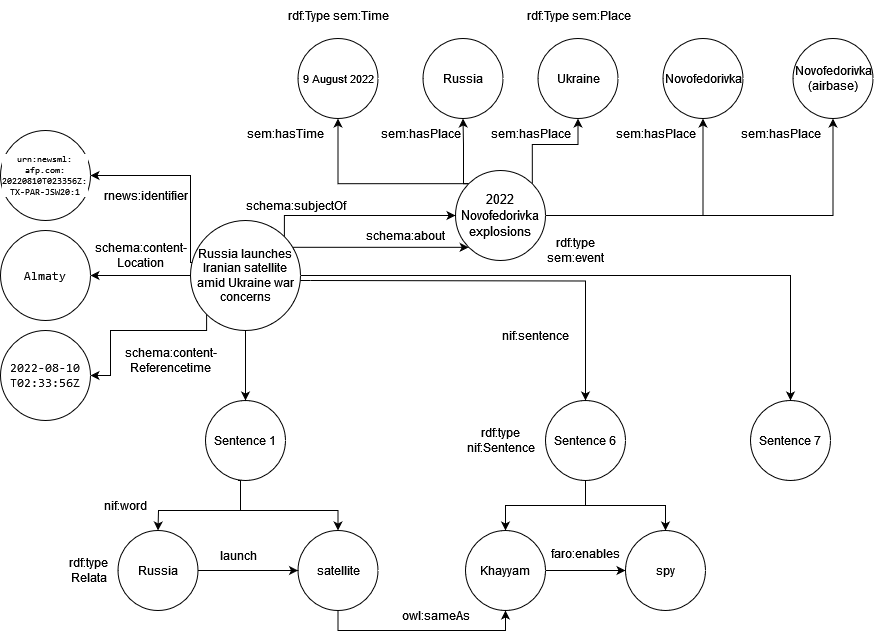
\includegraphics[scale=0.45]{Images/NG_article.png}
\caption{Part of the constructed narrative graph of the article "Russia launches Iranian satellite amid Ukraine war concerns"}
\label{fig:NG_article}
\end{sidewaysfigure}
\clearpage

\subsection{Overview Narrative Graph}
\begin{sidewaysfigure}[hb]
    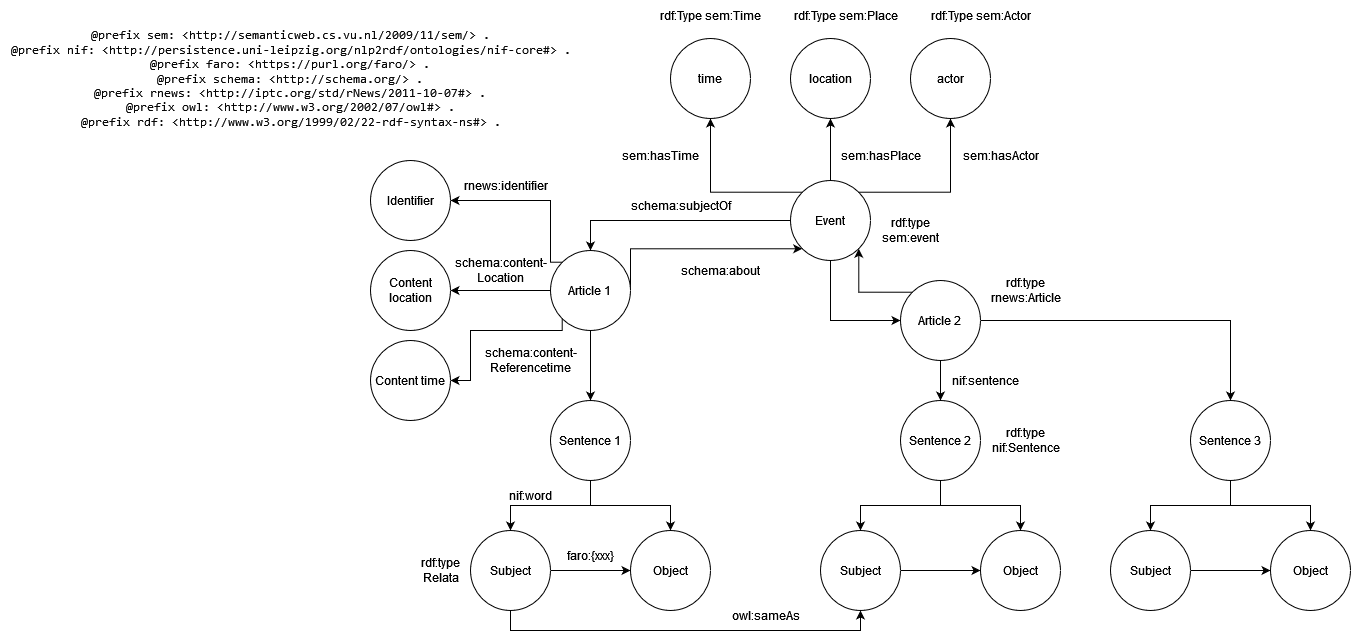
\includegraphics[scale=0.45]{Images/overview_graph.png}
\caption{Overview of the Narrative Graph}
\label{fig:graph_overview}
\end{sidewaysfigure}
% \clearpage


\end{document}

%%
%% End of file